\documentclass[12pt,a4paper]{book}

% $Id: pyvisi_doc.tex,v 1.3 2005/02/07 06:06:57 paultcochrane Exp $

%\setcounter{secnumdepth}{4}
%\setcounter{tocdepth}{4}

% $Id: pyvisi_defs.tex,v 1.2 2005/01/12 06:37:55 paultcochrane Exp $

\usepackage{html}
\usepackage{xspace}
% \usepackage{verbatim}  % better implementation of verbatim environment
\usepackage{alltt} % a verbatim-like environment that accepts commands
\usepackage{graphicx}
\usepackage{longtable} % handles long tables, stretching over multiple pages

%begin{latexonly}
%%%% I need the latexonly call here (even with the % signs, but
%%%% without the slash) as this
%%%% helps latex2html *not* see the stuff inbetween

% this code hacked from that of R Chandrasekhar from UWA
\newif\ifpdf
\ifx\pdfoutput\undefined
	\pdffalse    % we are not running pdfLaTeX
\else
	\pdfoutput=1 % we are running pdfLaTeX
	\pdftrue
\fi

% add the color package
\ifpdf
\usepackage[usenames,dvipsnames]{color}
\else
\usepackage[usenames,dvips]{color}
\fi

% add the hyperref package
\ifpdf
\usepackage[pdftex]{hyperref}
\else
\usepackage[hypertex]{hyperref}
\fi

% defines the colour for the background of code examples
\definecolor{LightGrey}{gray}{0.9}

\usepackage[grey,times]{quotchap}
\usepackage{ccaption}
\usepackage{fancyhdr}   

\ifpdf
	\DeclareGraphicsExtensions{.pdf}  % this command defined in graphicx
	\pdfcompresslevel=9  % 0: no compression, 9: highest compression
			     % or, set compress_level 9 in file pdftex.cfg
\else
	\DeclareGraphicsExtensions{.eps}
\fi

\setlength{\oddsidemargin}{-1in}   \setlength{\evensidemargin}{-1in}
\addtolength{\oddsidemargin}{25mm}\addtolength{\evensidemargin}{20mm}
\setlength{\marginparwidth}{40pt} \setlength{\marginparsep}{10pt}
\setlength{\topmargin}{-5mm}      \setlength{\headsep}{0.5in}
\setlength{\textheight}{227mm}    \setlength{\textwidth}{165mm}

\brokenpenalty=10000   % dunno what this does, maybe handy

% this stops one figure taking up a whole page and lets more text onto
% the one page when a figure exists
\renewcommand{\floatpagefraction}{0.8} %   Default = 0.5

% improved version of caption handling
\captionnamefont{\scshape}
\captionstyle{}
\makeatletter
\renewcommand{\fnum@figure}[1]{\quad\small\textsc{\figurename~\thefigure}:}
\renewcommand{\@makecaption}[2]{%
\vskip\abovecaptionskip
\sbox\@tempboxa{#1: #2}%
\ifdim \wd\@tempboxa >\hsize
  \def\baselinestretch{1}\@normalsize
  #1: #2\par
  \def\baselinestretch{1.5}\@normalsize
\else
  \global \@minipagefalse
  \hb@xt@\hsize{\hfil\box\@tempboxa\hfil}%
\fi
\vskip\belowcaptionskip}
\makeatother

\pagestyle{fancy}

%%%%% Fancyhdr stuff
% give the header a bit more room, otherwise LaTeX will spew on each page
\addtolength{\headheight}{2.5pt}
% define how headers are marked, for details, see fancyhdr docs
\renewcommand{\chaptermark}[1]{\markboth{#1}{}}
\renewcommand{\sectionmark}[1]{\markright{\thesection\ #1}}

% define where sections, chapters and pagenumbers are put
% see fancyhdr docs for details
% the \nouppercase stops book.cls making the contents, bibliography
% and index headers from being all in uppercase.
% The options used here are essentially that in Lamport's book, but
% with small caps for the headings.
\fancyhf{}
\fancyhead[LE,RO]{\nouppercase{\thepage}}
\fancyhead[LO]{\sc \nouppercase{\rightmark}}
\fancyhead[RE]{\sc \nouppercase{\leftmark}}

\bibliographystyle{apsrev}

% optional packages
\usepackage[square,comma,numbers,sort&compress]{natbib}
		% this is the natural sciences bibliography citation
		% style package.  The options here give citations in
		% the text as numbers in square brackets, separated by
		% commas, citations sorted and consecutive citations
		% compressed 
		% output example: [1,4,12-15]
		% should I make this optional and have unsrt as standard?

\usepackage[nottoc]{tocbibind}  
				% allows the table of contents, bibliography
				% and index to be added to the table of
				% contents if desired, the option used
				% here specifies that the table of
				% contents is not to be added.
				% tocbibind needs to be after natbib
				% otherwise bits of it get trampled.

\usepackage{amsmath,amsfonts,amssymb} % this is handy for mathematicians and physicists
			      % see http://www.ams.org/tex/amslatex.html

% \usepackage{showkeys} % this shows what labels you are using for cross
		      % references

% add the listings package to pretty print the code output
\usepackage{listings}
\begin{latexonly}
\lstdefinestyle{myC++}{%
%\lstset{%
language=C++,
showstringspaces=false,
basicstyle=\small\ttfamily,
commentstyle=\color[named]{BrickRed}\ttfamily,
keywordstyle=\color[named]{Purple}\ttfamily,
%identifierstyle=\color[named]{Blue}\ttfamily,
%functionstyle=\color[named]{Blue}\ttfamily,
%typestyle=\color[named]{ForestGreen}\ttfamily,
stringstyle=\color[named]{Tan}\ttfamily,%
morekeywords={,complex,}%
frame=none,%
backgroundcolor=\color{LightGrey}%
}

\lstdefinestyle{myMatlab}{%
%\lstset{%
language=Matlab,
showstringspaces=false,
basicstyle=\small\ttfamily,
commentstyle=\color[named]{BrickRed}\ttfamily,
keywordstyle=\color[named]{Purple}\ttfamily,
%identifierstyle=\color[named]{Blue}\ttfamily,
%functionstyle=\color[named]{Blue}\ttfamily,
%typestyle=\color[named]{ForestGreen}\ttfamily,
stringstyle=\color[named]{Tan}\ttfamily,%
frame=none,%
backgroundcolor=\color{LightGrey}%
}

\lstdefinestyle{myScilab}{%
%\lstset{%
language=Scilab,
showstringspaces=false,
basicstyle=\small\ttfamily,
commentstyle=\color[named]{BrickRed}\ttfamily,
keywordstyle=\color[named]{Purple}\ttfamily,
%identifierstyle=\color[named]{Blue}\ttfamily,
%functionstyle=\color[named]{Blue}\ttfamily,
%typestyle=\color[named]{ForestGreen}\ttfamily,
stringstyle=\color[named]{Tan}\ttfamily,%
frame=none,%
backgroundcolor=\color{LightGrey}%
}

\lstdefinestyle{myShell}{%
%\lstset{%
language=ksh,
showstringspaces=false,
basicstyle=\small\ttfamily,
commentstyle=\color[named]{Black}\ttfamily,
keywordstyle=\color[named]{Black}\ttfamily,
%identifierstyle=\color[named]{Blue}\ttfamily,
%functionstyle=\color[named]{Blue}\ttfamily,
%typestyle=\color[named]{ForestGreen}\ttfamily,
stringstyle=\color[named]{Black}\ttfamily,%
frame=none,%
backgroundcolor=\color{LightGrey}%
}

\lstdefinestyle{myPerl}{%
%\lstset{%
language=perl,
showstringspaces=false,
basicstyle=\small\ttfamily,
commentstyle=\color[named]{BrickRed}\ttfamily,
keywordstyle=\color[named]{Purple}\ttfamily,
%identifierstyle=\color[named]{Blue}\ttfamily,
%functionstyle=\color[named]{Blue}\ttfamily,
%typestyle=\color[named]{ForestGreen}\ttfamily,
stringstyle=\color[named]{Tan}\ttfamily,%
frame=none,%
backgroundcolor=\color{LightGrey}%
}

\lstdefinestyle{myPython}{%
%\lstset{%
language=python,
showstringspaces=false,
basicstyle=\small\ttfamily,
commentstyle=\color[named]{BrickRed}\ttfamily,
keywordstyle=\color[named]{Purple}\ttfamily,
%identifierstyle=\color[named]{Blue}\ttfamily,
%functionstyle=\color[named]{Blue}\ttfamily,
%typestyle=\color[named]{ForestGreen}\ttfamily,
stringstyle=\color[named]{Tan}\ttfamily,%
frame=none,%
backgroundcolor=\color{LightGrey}%
}
\end{latexonly}

%%%% I need the latexonly call here (even with the % signs, but
%%%% without the slash) as this
%%%% helps latex2html *not* see the stuff inbetween
%end{latexonly}

% put in an index?
\usepackage{makeidx}
\makeindex


% $Id: misc_defs.tex,v 1.3 2005/02/07 06:05:02 paultcochrane Exp $

\newcommand {\tbf}[1] {\textbf{#1}}
\newcommand {\tit}[1] {\textit{#1}}
\newcommand {\tmd}[1] {\textmd{#1}}
\newcommand {\trm}[1] {\textrm{#1}}
\newcommand {\tsc}[1] {\textsc{#1}}
\newcommand {\tsf}[1] {\textsf{#1}}
\newcommand {\tsl}[1] {\textsl{#1}}
\newcommand {\ttt}[1] {\texttt{#1}}
\newcommand {\tup}[1] {\textup{#1}}

\newcommand {\mbf}[1] {\mathbf{#1}}
\newcommand {\mmd}[1] {\mathmd{#1}}
\newcommand {\mrm}[1] {\mathrm{#1}}
\newcommand {\msc}[1] {\mathsc{#1}}
\newcommand {\msf}[1] {\mathsf{#1}}
\newcommand {\msl}[1] {\mathsl{#1}}
\newcommand {\mtt}[1] {\mathtt{#1}}
\newcommand {\mup}[1] {\mathup{#1}}

\newcommand {\figwidth} {100mm}
\newcommand {\Ref}[1] {Reference~\cite{#1}}
\newcommand {\Sec}[1] {Section~\ref{#1}}
\newcommand {\App}[1] {Appendix~\ref{#1}}
\newcommand {\Chap}[1] {Chapter~\ref{#1}}
\newcommand {\etal} {\emph{~et~al.}}
\newcommand {\bul} {$\bullet$ }   % bullet
\newcommand {\fig}[1] {Figure~\ref{#1}}   % references Figure x
\newcommand {\imp} {$\Rightarrow$}   % implication symbol (default)
\newcommand {\impt} {$\Rightarrow$}   % implication symbol (text mode)
\newcommand {\impm} {\Rightarrow}   % implication symbol (math mode)
\newcommand {\vect}[1] {\mathbf{#1}} 
%\renewcommand {\vec}[1] {\mathbf{#1}}
\newcommand {\hvect}[1] {\hat{\mathbf{#1}}}
\newcommand {\del} {\partial}
\newcommand {\eqn}[1] {Equation~(\ref{#1})} 
\newcommand {\tab}[1] {Table~\ref{#1}} % references Table x
\newcommand {\half} {\frac{1}{2}} 

%%%%% pyvisi stuff

% pyvisi version and release number commands
\newcommand{\pyvisiVersionNo}{0.1}
\newcommand{\pyvisiReleaseNo}{pre-alpha-1}
\newcommand{\pyvisiVersion}{\pyvisiVersionNo-\pyvisiReleaseNo}

\newcommand {\pyvisi} {\tbf{PyVisi}\xspace}

% this implements nicely formatted shell code in the latex and html
% versions of the document
%begin{latexonly}
\lstnewenvironment{shellCode}[1][]{\lstset{style=myShell}\lstset{#1}}{}
%end{latexonly}
\begin{htmlonly}
\newenvironment{shellCode}{\begin{alltt}}{\end{alltt}}
\end{htmlonly}

% this implements nicely formatted Perl code in the latex and html
% versions of the document
%begin{latexonly}
\lstnewenvironment{perlCode}[1][]{\lstset{style=myPerl}\lstset{#1}}{}
%end{latexonly}
\begin{htmlonly}
\newenvironment{shellCode}{\begin{alltt}}{\end{alltt}}
\end{htmlonly}

% this implements nicely formatted Python code in the latex and html
% versions of the document
%begin{latexonly}
\lstnewenvironment{pythonCode}[1][]{\lstset{style=myPython}\lstset{#1}}{}
%end{latexonly}
\begin{htmlonly}
\newenvironment{shellCode}{\begin{alltt}}{\end{alltt}}
\end{htmlonly}

% this implements nicely formatted C++ code in the latex and html
% versions of the document
%begin{latexonly}
\lstnewenvironment{CCode}{\lstset{style=myC++}}{}
%end{latexonly}
\begin{htmlonly}
\newenvironment{CCode}{\begin{alltt}}{\end{alltt}}
\end{htmlonly}

% this implements nicely formatted matlab code in the latex and html
% versions of the document
%begin{latexonly}
\lstnewenvironment{matlabCode}{\lstset{style=myMatlab}}{}
%end{latexonly}
\begin{htmlonly}
\newenvironment{matlabCode}{\begin{alltt}}{\end{alltt}}
\end{htmlonly}

% this implements nicely formatted scilab code in the latex and html
% versions of the document
%begin{latexonly}
\lstnewenvironment{scilabCode}{\lstset{style=myScilab}}{}
%end{latexonly}
\begin{htmlonly}
\newenvironment{scilabCode}{\begin{alltt}}{\end{alltt}}
\end{htmlonly}

\newcommand{\textarrow}{$\rightarrow$\xspace}
\newcommand{\forcenewline}{\rule{2ex}{0pt}\\}
\newcommand{\reqd}{\textit{required}\xspace}
\newcommand{\optl}{\textit{optional}\xspace}
\newenvironment{pyvisiDoc}{\begin{tabular}{ll}%
\rule{0pt}{10ex}\hspace*{5mm} &%
\begin{minipage}{15cm}\small%
\begin{description}}
{\end{description}\normalsize%
\end{minipage}%
\end{tabular}\vfill}

% spell things correctly
\newenvironment{centre}{\begin{center}}{\end{center}}
\newenvironment{itemise}{\begin{itemize}}{\end{itemize}}



\begin{document}

\frontmatter

% $Id: titlepage.tex,v 1.2 2005/02/07 06:36:01 paultcochrane Exp $

\title{\Huge \pyvisi --- {\Large The Python Visualisation Interface}}

%\centerline{\Large Version \pyvisiVersion}

\author{P.~T.~Cochrane}

\maketitle

% $Id: abstract.tex,v 1.3 2005/02/07 06:01:26 paultcochrane Exp $

\chapter*{Abstract}

\section*{About this manual}

This manual has been split into five parts in an attempt to cover all of the
material necessary to be able to use and master \pyvisi, but also to provide an
entry point for novices and experts alike.

Part~\ref{part:tutorial} is a very simple introduction to \pyvisi, and
discusses how to use \pyvisi to visualise ones data.  Novice users may wish to
start with \Chap{chap:tutFromScratch} (Starting from scratch) to help
themselves get going with \pyvisi.  

Part~\ref{part:userManual} gives user-level information about \pyvisi and
generic ideas behind the interface and how to use it (well, hopefully in the
future anyway).

Part~\ref{part:languageReference} gives specific information about the objects
and methods available for use in \pyvisi.  For renderer-specific documenation
see either the relevant section of this manual (to come) or the renderer
module's own documentation.

Part~\ref{part:developerManual} gives developer-level information on what
developers of renderer modules need to provide, and how they can do it.

Part~\ref{part:appendix} is an appendix and will cover any extra items of
interest, and includes the GNU General Public License, and a bibliography.

\section*{Tools used to build \pyvisi}

These are the multifarious tools with which \pyvisi, its documentation (both
handmade and automatically generated) and its web pages, has been made.

\begin{itemize}
\item General development tools: cvs, aap, dia, pyscript, pylint
\item Editors: emacs, vim
\item Linux Distributions: Gentoo Linux, Fedora Linux
\item Scripting tools and languages: \htmladdnormallink{python}{http://www.python.org}~\cite{web:python}
\item Documentation tools: \LaTeX, latex2html, epydoc, doxygen
\item Organisations: sourceforge.net, ESSCC, ACcESS
\end{itemize}

\section*{Feedback}

Yes, we want feedback!  If you have any comments about \pyvisi and/or this
manual (such as, inaccuracies, possible improvements, new features, what it
does well, etc.) then please email one of the current developer or the \pyvisi
web page webmaster.  You can find the addresses of both of these people on the
\pyvisi web page: \htmladdnormallink{http://pyvisi.sourceforge.net}
{http://pyvisi.sourceforge.net}.  And please, feel free to mention anything, no
matter how small.  It would be great to see \pyvisi improve the way people
want, and for it to be documented the way the \pyvisi user community wants.

\tableofcontents
%\listoffigures
%\listoftables

\mainmatter

\part{Tutorial}
\label{part:tutorial}

% $Id: tutFromScratch.tex,v 1.2 2005/01/12 04:05:36 paultcochrane Exp $

\chapter{Starting from scratch}
\label{chap:tutFromScratch}

A first go at a \pyvisi script.


\part{User Manual}
\label{part:userManual}

%%%%%%%%%%%%%%%%%%%%%%%%%%%%%%%%%%%%%%%%%%%%%%%%%%%%%%%%
%
% Copyright (c) 2003-2009 by University of Queensland
% Earth Systems Science Computational Center (ESSCC)
% http://www.uq.edu.au/esscc
%
% Primary Business: Queensland, Australia
% Licensed under the Open Software License version 3.0
% http://www.opensource.org/licenses/osl-3.0.php
%
%%%%%%%%%%%%%%%%%%%%%%%%%%%%%%%%%%%%%%%%%%%%%%%%%%%%%%%%

\documentclass{manual}

%%%%%%%%%%%%%%%%%%%%%%%%%%%%%%%%%%%%%%%%%%%%%%%%%%%%%%%%
%
% Copyright (c) 2003-2008 by University of Queensland
% Earth Systems Science Computational Center (ESSCC)
% http://www.uq.edu.au/esscc
%
% Primary Business: Queensland, Australia
% Licensed under the Open Software License version 3.0
% http://www.opensource.org/licenses/osl-3.0.php
%
%%%%%%%%%%%%%%%%%%%%%%%%%%%%%%%%%%%%%%%%%%%%%%%%%%%%%%%%

% Please do not use .ps only packages.
% As a minimum this document should build under pdflatex

\usepackage{color}
\usepackage{xspace}

%Ensures that latex doesn't have an error if we don't specify the version
\providecommand{\RepVersion}{Unknown\xspace}
% to set this value use:
% (pdf)latex '\newcommand{\RepVersion}{version\xspace}%%%%%%%%%%%%%%%%%%%%%%%%%%%%%%%%%%%%%%%%%%%%%%%%%%%%%%%%
%
% Copyright (c) 2003-2009 by University of Queensland
% Earth Systems Science Computational Center (ESSCC)
% http://www.uq.edu.au/esscc
%
% Primary Business: Queensland, Australia
% Licensed under the Open Software License version 3.0
% http://www.opensource.org/licenses/osl-3.0.php
%
%%%%%%%%%%%%%%%%%%%%%%%%%%%%%%%%%%%%%%%%%%%%%%%%%%%%%%%%

\documentclass{manual}

\input{install_defs}

\title{Installation guide for Escript and Finley}

\author{Escript development team}
\authoraddress{
Earth Systems Science Computational Centre (ESSCC) \\
The University of Queensland \\
Brisbane, Australia \\
Email: \email{esys@esscc.uq.edu.au}
}
\date{\today}      
\release{Revision: \RepVersion}
\setreleaseinfo{development version} 
\setshortversion{\RepVersion}

\makeindex
\begin{document}

\maketitle
\tableofcontents

\include{intro}
\include{bincommon}		% material common to all binary installs
\include{binmac}
\include{binwin}
\chapter{Building escript from source}
\label{chap:essrc}
\input{srcommon}		% material common to all source installs
\include{allsrccommon} 
\end{document}
'
% as your command-line

%\usepackage[colorlinks=true, pdftitle={Escript/Finley install guide}, pdfauthor={Escript development team}
%,pdfpagelayout=TwoColumnRight]{hyperref}
\usepackage{listings}        % add the listings package to pretty print the code output


% Try to make this the last \usepackage
%\usepackage[colorlinks=true, pdftitle={Escript/Finley install guide}, pdfauthor={Escript development team}
%,pdfpagelayout=TwoColumnRight]{hyperref}

\newcommand{\escript}{\module{esys.escript}\xspace}
\newcommand{\finley}{\module{esys.finley}\xspace}
\newcommand{\esys}{\module{esys}\xspace}

\newcommand{\esfinley}{Escript/Finley\xspace}
\newcommand{\linux}{Linux\xspace}
\newcommand{\macosx}{MacOS~X\xspace}
\newcommand{\winxp}{Windows~XP\xspace}
\newcommand{\openmp}{OpenMP\xspace}
\newcommand{\mpi}{MPI\xspace}

\newcommand{\Sec}[1] {Section~\ref{#1}}
\newcommand*{\filename}[1]{\texttt{#1}\xspace}

% defines the colour for the background of code examples
\definecolor{LightGrey}{gray}{0.9}


\lstdefinestyle{myShell}{%
%\lstset{%
language=ksh,
showstringspaces=false,
basicstyle=\small\ttfamily,
commentstyle=\color{black}\ttfamily,
keywordstyle=\color{black}\ttfamily,
%identifierstyle=\color[named]{Blue}\ttfamily,
%functionstyle=\color[named]{Blue}\ttfamily,
%typestyle=\color[named]{ForestGreen}\ttfamily,
stringstyle=\color{black}\ttfamily,%
frame=none,%
backgroundcolor=\color{LightGrey}%
}

% this implements nicely formatted shell code
\lstnewenvironment{shellCode}[1][]{\lstset{style=myShell}\lstset{#1}}{}

\newcommand{\todo}[1]{\emph{TODO:}{\em #1}}



\title{Installation guide for Escript and Finley}

\author{Escript development team}
\authoraddress{
Earth Systems Science Computational Centre (ESSCC) \\
The University of Queensland \\
Brisbane, Australia \\
Email: \email{esys@esscc.uq.edu.au}
}
\date{\today}      
\release{Revision: \RepVersion}
\setreleaseinfo{development version} 
\setshortversion{\RepVersion}

\makeindex
\begin{document}

\maketitle
\tableofcontents



%%%%%%%%%%%%%%%%%%%%%%%%%%%%%%%%%%%%%%%%%%%%%%%%%%%%%%%%
%
% Copyright (c) 2003-2008 by University of Queensland
% Earth Systems Science Computational Center (ESSCC)
% http://www.uq.edu.au/esscc
%
% Primary Business: Queensland, Australia
% Licensed under the Open Software License version 3.0
% http://www.opensource.org/licenses/osl-3.0.php
%
%%%%%%%%%%%%%%%%%%%%%%%%%%%%%%%%%%%%%%%%%%%%%%%%%%%%%%%%

This document describes how to install \esfinley on your computer.
To learn how to use \esfinley please see the User guide or, for
more detailed information, the API documentation.
%%%%%%%%%%%%%%%%%%%%%%%%%%%%%%%%%%%%%%%%%%%%%%%%%%%%%%%%%%%%%%%%%%%%%%%%%%%%%%
% Copyright (c) 2003-2013 by University of Queensland
% http://www.uq.edu.au
%
% Primary Business: Queensland, Australia
% Licensed under the Open Software License version 3.0
% http://www.opensource.org/licenses/osl-3.0.php
%
% Development until 2012 by Earth Systems Science Computational Center (ESSCC)
% Development since 2012 by School of Earth Sciences
%
%%%%%%%%%%%%%%%%%%%%%%%%%%%%%%%%%%%%%%%%%%%%%%%%%%%%%%%%%%%%%%%%%%%%%%%%%%%%%%

% material common to all binary distributions.

\chapter{Binary releases}\label{chap:bin}

Binary distributions (no compilation required) are available for the following operating systems:
\begin{itemize}
 \item \linux~-- Section~\ref{sec:binlinux}
 \item \macosx~-- Section~\ref{sec:binmac}
 \item Windows~-- Section~\ref{sec:binwin}.
\end{itemize}

Note that only the Debian/Ubuntu binary packages support \openmp and \mpi.
If you need these features you will need to compile \esfinley from source (see Section~\ref{sec:compilesrc} 
and Section~\ref{sec:compileescriptlinux}.)


%%%%%%%%%%%%%%%%%%%%%%%%%%%%%%%%%%%%%%%%%%%%%%%%%%%%%%%%
%
% Copyright (c) 2003-2010 by University of Queensland
% Earth Systems Science Computational Center (ESSCC)
% http://www.uq.edu.au/esscc
%
% Primary Business: Queensland, Australia
% Licensed under the Open Software License version 3.0
% http://www.opensource.org/licenses/osl-3.0.php
%
%%%%%%%%%%%%%%%%%%%%%%%%%%%%%%%%%%%%%%%%%%%%%%%%%%%%%%%%

\section{Linux binary installation}
\label{sec:binlinux}

\esfinley can be installed as a stand-alone bundle, containing all the required dependencies.
Alternatively, if we have a package for your distribution you can use the standard tools to install.


For more information on using the \file{run-escript} command please see the User's Guide.

If you are using Debian~5.0(``Lenny''), Ubuntu~8.10(``Intrepid Ibex'') or greater, then see Section~\ref{sec:debian}.
For other linux distributions refer to Section~\ref{sec:standalonelinux}.

\subsection{Debian and Ubuntu}\label{sec:debian}

At the time of this writing we only produce deb's for the i386 and amd64 architectures.
The package file will be named \file{escript-X-D_A.deb} where \texttt{X} is the version, \texttt{D} is the distribution codename (eg ``\texttt{lenny}'' or ``\texttt{jaunty}'') and \texttt{A} is the architecture.
For example, \file{escript-3.0-1-lenny_amd64.deb} would be the file for lenny for 64bit processors.
To install \esfinley download the appropriate \file{.deb} file and execute the following commands as root (you need to be in the directory containing the file):

\begin{verse}
\textbf{(For users of Ubuntu~10.10 \textit{``Maverick Meercat''} only)}\\
You will need to either install \texttt{aptitude}\footnote{Unless you are short on disk space \texttt{aptitude} is recommended} or replace use \texttt{apt-get} where this guide uses \texttt{aptitude}.
\begin{shellCode}
sudo apt-get install aptitude
\end{shellCode}
\end{verse}

\begin{shellCode}
dpkg --unpack escript*.deb
aptitude install escript
\end{shellCode}

Installing escript should not remove any packages from your system.
If aptitude suggests removing escript, then choose 'N'.
It should then suggest installing some dependencies choose 'Y' here.
If it suggests removing escript-noalias then agree.

If you use sudo (for example on Ubuntu) enter the following instead:
\begin{shellCode}
sudo dpkg --unpack escript*.deb
sudo aptitude install escript
\end{shellCode}

This should install \esfinley and its dependencies on your system.
Please notify the development team if something goes wrong.

\subsection{Stand-alone bundle}\label{sec:standalonelinux}

If there is no package available for your distribution, you may be able to use one of our stand alone bundles.
These come in two parts: escript itself (\file{escript_3.2_i386.tar.bz2}) and a group of required programs (\file{escript-support_3.0_i386.tar.bz2}) (Note that the support bundle is version~3.0 not 3.2) . For $64$-bit Intel and Amd processors substitute \texttt{amd64} for \texttt{i386}.
This point release uses the same support bundle as previous releases so if you already have it you don't need a new version.
\begin{shellCode}
tar -xjf escript-support_3.0_i386.tar.bz2
tar -xjf escript_3.2_i386.tar.bz2
\end{shellCode}
This will produce a directory called \file{stand} which contains a stand-alone version of \esfinley and its dependencies.
You can rename or move it as is convenient to you, no installation is required.
Test your installation by running:
\begin{shellCode}
stand/escript.d/bin/run-escript
\end{shellCode}
This should give you a normal python shell.
If you wish to save on typing you can add \file{x/stand/escript.d/bin}\footnote{or whatever you renamed \texttt{stand} to.} to your \texttt{PATH} variable (where x is the absolute path to your install).


		% material common to all binary installs
%%%%%%%%%%%%%%%%%%%%%%%%%%%%%%%%%%%%%%%%%%%%%%%%%%%%%%%%%%%%%%%%%%%%%%%%%%%%%%
% Copyright (c) 2003-2012 by University of Queensland
% http://www.uq.edu.au
%
% Primary Business: Queensland, Australia
% Licensed under the Open Software License version 3.0
% http://www.opensource.org/licenses/osl-3.0.php
%
% Development until 2012 by Earth Systems Science Computational Center (ESSCC)
% Development since 2012 by School of Earth Sciences
%
%%%%%%%%%%%%%%%%%%%%%%%%%%%%%%%%%%%%%%%%%%%%%%%%%%%%%%%%%%%%%%%%%%%%%%%%%%%%%%

\section{\macosx binary installation}
\label{sec:binmac}

The standalone release for OSX has been tested on \macosx 10.5 (``Leopard'')\footnote{It \emph{should} work on 
``Snow Leopard'' but has not been tested.} and 10.7 (``Lion'').

You will need to download both escript (\file{escript_3.4_osx.dmg}) and the support files (\file{escript-support_3.0_osx.dmg}).
This point release uses the same support bundle as previous releases so if you already have it you don't need a new version.
You will also need to download the sympy source code from \url{sympy.org} (You are looking for a \texttt{.tar.gz} file).

\begin{itemize}
\item Create a folder to hold escript (no spaces in the name please).
\item Open the \file{.dmg} files and copy the contents to the folder you just created.
\item Copy the sympy file into the same directory.
\end{itemize}

To use escript, open a terminal\footnote{If you do not know how to open a terminal on Mac, then just type \texttt{terminal} in the spotlight (search tool on the top of the right corner) and once found, just click on it.} and type
\begin{shellCode}
eval `x/escript.d/bin/run-escript -e`
\end{shellCode}
where \textit{x} is the absolute path to your install.

\noindent Now we need to install sympy (substitue the version number of sympy you have):
\begin{shellCode}
tar -xzf sympy-0.7.1.tar.gz
cd sympy-0.7.1
python setup.py install --prefix ../stand/pkg
\end{shellCode}

You cay test your install with:
\begin{shellCode}
run-escript
\end{shellCode}

You may now remove the sympy files from the starting directory and ``eject'' the \texttt{.dmg} files.

If you wish to save on typing you can add \file{x/escript.d/bin} to your PATH variable 
(where \textit{x} is the absolute path to your install). 



%%%%%%%%%%%%%%%%%%%%%%%%%%%%%%%%%%%%%%%%%%%%%%%%%%%%%%%%
%
% Copyright (c) 2003-2008 by University of Queensland
% Earth Systems Science Computational Center (ESSCC)
% http://www.uq.edu.au/esscc
%
% Primary Business: Queensland, Australia
% Licensed under the Open Software License version 3.0
% http://www.opensource.org/licenses/osl-3.0.php
%
%%%%%%%%%%%%%%%%%%%%%%%%%%%%%%%%%%%%%%%%%%%%%%%%%%%%%%%%

\section{Windows binary installation}
\label{sec:binwin}

There is no automated install/uninstall procedure for \escript on Windows at this time.
However, the following procedure appears to work for the previous release\footnote{Thanks to Peter Hornby and Frederick Roger for this report.}

Please ensure you have the following software installed: 
\begin{itemize}
 \item pythonxy (\url{http://www.pythonxy.com})
%\item numarray 1-5-2win32py2.5  for  win32
\end{itemize}

From the escript zip file:
\begin{itemize}
\item 
 copy the \filename{esys} directory to your Python 2.5 site-packages folder (usually \filename{C:\textbackslash Python25\textbackslash Lib\textbackslash site-packages}).
\item 
 copy the \filename{.dll} files from \filename{esys\_dlls} to a directory on your PATH. For example copy the directory to \filename{C:\textbackslash Python25\textbackslash libs\textbackslash esys\_dlls} and add  \filename{C:\textbackslash Python25\textbackslash libs\textbackslash esys\_dlls} to your PATH.
\end{itemize}


\chapter{Building escript from source}
\label{chap:essrc}
%%%%%%%%%%%%%%%%%%%%%%%%%%%%%%%%%%%%%%%%%%%%%%%%%%%%%%%%
%
% Copyright (c) 2003-2009 by University of Queensland
% Earth Systems Science Computational Center (ESSCC)
% http://www.uq.edu.au/esscc
%
% Primary Business: Queensland, Australia
% Licensed under the Open Software License version 3.0
% http://www.opensource.org/licenses/osl-3.0.php
%
%%%%%%%%%%%%%%%%%%%%%%%%%%%%%%%%%%%%%%%%%%%%%%%%%%%%%%%%

% This file contains material common to all src distributions.

% The original version of this content came from the esscc twiki page maintained by ksteube

This chapter describes how to build \esfinley from source assuming that the dependencies are already installed (for example using precompiled packages for your OS).
\Sec{sec:deps} describes the dependencies, while \Sec{sec:compilesrc} gives the compile instructions.

If you would prefer to build all the dependecies from source in the escript-support packages please see \Chap{chap:allsrc}.
\esfinley is known to compile and run on the following systems:
\begin{itemize}
 \item \linux using gcc\footnote{There are some problems with \openmp under gcc prior to version 4.3.2. Also do not link the gomp library with gcc 4.3.3 - it causes problems.}
\item \linux using icc on SGI ICE 8200
\item \macosx using gcc
\item \winxp using the Visual C compiler (we do not specifically discuss Windows builds in this guide).
\end{itemize}

\section{External dependencies}
\label{sec:deps}
The following external packages are required in order to compile and run \esfinley.
Where version numbers are specified, more recent versions can probably be subsituted.
You can either try the standard/precompiled packages available for your operating system or you can download and build them from source.
The advantage of using existing packages is that they are more likely to work together properly.
You must take greater care if downloading sources separately.

\begin{itemize}
 \item python-2.5.1 (\url{http://python.org}) \\-
        Python interpreter (you must compile with shared libraries.)
 \item numpy 1.1.0 (\url{http://numpy.scipy.org}) \\-
        Arrays for python
 \item boost-1.35 (\url{http://www.boost.org}) \\-
        Interface between C++ and Python
 \item scons-0.989.5 (\url{http://www.scons.org/}) \\-
        Python-based alternative to ``make''.
\end{itemize}

The version numbers given here are not strict requirements, more recent (and in some cases older) versions are very likely to work.
The following packages should be sufficient (but not necessarily minimal) for Debian 5.0 (``Lenny''):
python-dev, libboost1.35-dev, scons, python-numpy, g++.

These packages may be required for some of the optional capabilities of the system:

\begin{itemize}
 \item netcdf-3.6.2 (\url{http://www.unidata.ucar.edu/software/netcdf}) \\-
        Used to save data sets in binary form for checkpoint/restart (must be compiled with -fPIC)
 \item vtk-5.0.4 (\url{http://www.vtk.org}) \\-
        Used to save VTK files for visualization
  \begin{itemize}
   \item cmake-2.4.6 (\url{http://www.cmake.org}) \\-
        Required to build VTK
   \item mesa-7.0.3 (\url{http://www.mesa3d.org})\\-
        Free OpenGL replacement used by VTK
  \end{itemize}
 \item netpbm (\url{http://netpbm.sourceforge.com}) \\-
        Tools for producing movies from images
 \item mpich2-1.0.7 (\url{http://www.mcs.anl.gov/research/projects/mpich2}) \\-
        Parallelization with \mpi
 \item parmetis-3.1 (\url{http://glaros.dtc.umn.edu/gkhome/metis/parmetis/overview}) \\-
        Optimization of the stiffness matrix
 \item MKL \\(\url{http://www.intel.com/cd/software/products/asmo-na/eng/307757.htm}) \\-
        Intel's Math Kernel Library for use with their C compiler.
\end{itemize}

The following packages might be useful for mesh generation:
\begin{itemize}
 \item gmsh-2.2.0 (\url{http://www.geuz.org/gmsh}) \\-
        Mesh generation and viewing
  \begin{itemize}
   \item fltk-1.1.9 (\url{http://www.fltk.org}) \\-
        Required to build gmsh 
   \item gsl-1.10 (\url{http://www.gnu.org/software/gsl}) \\-
        Required to build gmsh 
  \end{itemize}
 \item triangle-1.6 (\url{http://www.cs.cmu.edu/~quake/triangle.html}) \\-
        Two-dimensional mesh generator and Delaunay triangulator.
\end{itemize}

Packages for visualization:
\begin{itemize}
 \item mayavi-1.5 (\url{http://mayavi.sourceforge.net}) \\-
        MayaVi is referenced in our User's Guide for viewing VTK files
 \item visit-1.11.2 (\url{https://wci.llnl.gov/codes/visit/}) \\-
        A featureful visualization system with movie-making capabilities.
\end{itemize}

\section{Compilation}\label{sec:compilesrc}
Throughout this section we will assume that the source code is uncompressed in a directory called \filename{escript.d}.
You can call the directory anything you like, provided that you make the change before you compile.

You need to indicate where to find the external dependencies.
Unless specified otherwise, all paths will be relative to the top level of the source.
To do this, create a file in the \filename{scons} directory called \filename{x_options.py} where ``x'' is the name of your computer (output of the \texttt{hostname} command).
As a starting point use one of the following:
\begin{itemize}
 \item \filename{scons/linux_options_example.py} (\linux desktop)
\item \filename{scons/mac_options_example.py} (\macosx desktop)
\item \filename{ice_options_example.py} (SGI ICE 8200)
\item \filename{winxp_options_example.py} (\winxp)
\end{itemize}

To actually compile (if you have $n$ processors, then you can use \texttt{scons -j$n$} instead):

\begin{shellCode}
cd escript.d
scons
\end{shellCode}

As part of its output, scons will tell you the name of the options file it used as well as a list of features 
and whether they are enabled for your build.

If you require debug versions of the libraries, use:
\begin{shellCode}
 scons usedebug=yes
\end{shellCode}
A note about scons: if you recompile later with different options (e.g. leaving out usedebug), scons will revert 
to its default values. If you wish to make a change more permanent, then modify your options file.


You can install the binaries/libraries in a different location with:
\begin{shellCode}
 scons prefix=some_dir
\end{shellCode}

You can test your build using 
\begin{shellCode}
scons all_tests
\end{shellCode}
Grab a coffee or two while the tests compile and run.
An alternative method is available for performing tests on \openmp and \mpi builds.

\subsection{Compilation with \openmp}
You will need to consult your compiler documentation for the precise switches to use to enable \openmp features.
Once you know the options, modify the omp_optim, omp_debug and omp_libs variables in your options.py file.

For example, for gcc compilers which support \openmp use:
\begin{shellCode}
omp_optim		= '-fopenmp'
omp_debug		= '-fopenmp'
omp_libs		= ['gomp']
\end{shellCode}
Depending on your version, the last change may not be required.
If you're unsure try without the gomp library first and add it if you get linker errors.

Then recompile.
\begin{shellCode}
 scons useopenmp=yes
\end{shellCode}

You can test your build, e.g. using 4 threads by issuing
\begin{shellCode}
export ESCRIPT_NUM_THREADS=4
scons all_tests
\end{shellCode}

\subsection{Compilation with \mpi}
You will need to have \mpi installed on your system.
There are a number of implementations so we do not provide any specific advice here.
You will need to modify the following variables in your options file.
\begin{itemize}
 \item \texttt{mpi_flavour} \\
	which \mpi implementation is used. Valid values are
    \begin{itemize}
        \item[\texttt{MPT}] SGI MPI implementation \\
            \url{http://techpubs.sgi.com/library/manuals/3000/007-3687-010/pdf/007-3687-010.pdf}
        \item[\texttt{MPICH2}] Argonne's MPICH version 2 implementation \\
            \url{http://www.mcs.anl.gov/research/projects/mpi/mpich2/}
        \item[\texttt{MPICH}] Argonne's MPICH implementation \\
            \url{http://www.mcs.anl.gov/research/projects/mpi/mpich1/}
        \item[\texttt{OPENMPI}] Open MPI \\
            \url{http://www.open-mpi.org/}
        \item[\texttt{INTELMPI}] Intel's MPI \\
            \url{http://software.intel.com/en-us/intel-mpi-library/}
    \end{itemize}
 \item \texttt{mpi_path} \\
	where to find \filename{mpi.h}
 \item \texttt{mpi_lib_path} \\
	where to find libraries for \mpi
 \item \texttt{mpi_libs} \\
	which libraries to link to.
\end{itemize}

Then compile with:
\begin{shellCode}
 scons usempi=yes
\end{shellCode}

As with debug and openmp, you can make this a more permanent setting by modifying your options file.

To test your build using 6 processors enter:
\begin{shellCode}
export ESCRIPT_NUM_NODES=6
scons usempi=yes all_tests
\end{shellCode}
and on 6 processors with 4 threads each using 
\begin{shellCode}
export ESCRIPT_NUM_THREADS=4
export ESCRIPT_NUM_NODES=6
scons usempi=yes all_tests
\end{shellCode}
Alternatively, you can give a hostfile
\begin{shellCode}
export ESCRIPT_NUM_THREADS=4
export ESCRIPT_HOSTFILE=myhostfile
scons usempi=yes all_tests
\end{shellCode}
Note that depending on your \mpi flavour it may be required to start a daemon before running the tests under \mpi.


\subsection{Difficulties}

%This is copied from Ken's notes on the old Twiki page
\subsubsection{``Bad magic number''}
This error usually indicates that the version of python used to run escript differs from the version used when installing escript (Use \texttt{which python} and \texttt{python --version} to check).

It is also possible that incompatible libraries were used when compiling \esfinley.
For example, if you run with Python2.4 but the software was compiled against Python2.5 then you will get unsatisfied externals or a large error message with a long traceback.
Another case is when Boost or Numarray was compiled against the wrong Python library.
To avoid these problems both builder and user must ensure they are using the same python libraries.

\subsubsection{\openmp builds segfault running examples}

One known cause for this is linking the \filename{gomp} library with escript built using gcc 4.3.3.
While you need the \texttt{-fopenmp} switch you should not need to link \filename{gomp}.

		% material common to all source installs
%%%%%%%%%%%%%%%%%%%%%%%%%%%%%%%%%%%%%%%%%%%%%%%%%%%%%%%%%%%%%%%%%%%%%%%%%%%%%%
% Copyright (c) 2003-2012 by University of Queensland
% http://www.uq.edu.au
%
% Primary Business: Queensland, Australia
% Licensed under the Open Software License version 3.0
% http://www.opensource.org/licenses/osl-3.0.php
%
% Development until 2012 by Earth Systems Science Computational Center (ESSCC)
% Development since 2012 by School of Earth Sciences
%
%%%%%%%%%%%%%%%%%%%%%%%%%%%%%%%%%%%%%%%%%%%%%%%%%%%%%%%%%%%%%%%%%%%%%%%%%%%%%%

\chapter{Building escript and dependencies from source}
\label{chap:allsrc}

This chapter describes how to build escript and its dependencies from the source code in the escript support packages.
You can also use these instructions if you have gathered the various sources yourself.
Section~\ref{sec:addfunc} lists additional visualisation tools.

%%%%%%%%%%%%%%%%%%%%%%%%%%%%%%%%%%%%%%%%%%%%%%%%%%%%%%%%
%
% Copyright (c) 2003-2009 by University of Queensland
% Earth Systems Science Computational Center (ESSCC)
% http://www.uq.edu.au/esscc
%
% Primary Business: Queensland, Australia
% Licensed under the Open Software License version 3.0
% http://www.opensource.org/licenses/osl-3.0.php
%
%%%%%%%%%%%%%%%%%%%%%%%%%%%%%%%%%%%%%%%%%%%%%%%%%%%%%%%%

\section{Installing from source for \linux}
\label{sec:srclinux}

\subsection{Preliminaries}

The following instructions assume you are running the \filename{bash} shell.
Comments are indicated with \# characters.

Make sure you have the following installed:
\begin{itemize}
 \item \filename{g++} and associated tools.
 \item \filename{make}
 % I suspect that these are only needed by VTK and if we aren't using it anymore they could be removed
%  \item \filename{libXext.so}\footnote{In Debian this is in the libXext-dev package.}
%  \item \filename{libxt.so}\footnote{In Debian this is in the libxt-dev package.}
\end{itemize}

To compile matplotlib you will also need the following\footnote{For Debian and Ubuntu users, installing \filename{libfreetype6-dev} and \filename{libpng-dev} will be sufficient.} (if your distribution separates development files,
make sure to get the development packages):
\begin{itemize}
 \item \filename{freetype2}
\item \filename{zlib}
\item \filename{libpng}
\end{itemize}



You will also need a copy of the \esfinley source code.
If you retrieved the source using subversion, don't forget that one can use the export command instead of checkout to get a smaller copy.
For additional visualization functionality see \Sec{sec:addfunc}.

These instructions will produce the following directory structure:
\begin{itemize}
 \item[] \filename{stand} \begin{itemize}
  \item[] \filename{escript.d}
  \item[] \filename{pkg}
  \item[] \filename{pkg_src}
  \item[] \filename{build}
  \item[] \filename{doc}
 \end{itemize}
\end{itemize}

Before you start copy the \esfinley source into the \filename{escript.d} directory.
The following instructions refer to software versions in the \filename{escript-support-3-src} bundle.
If you download your own versions of those packages substitute their version numbers and names as appropriate.
There are a number of uses of the \filename{make} command in the following instructions.
If your computer has multiple cores/processors you can speed up the compilation process by adding -j 2 after the make command.
For example to use all processors on a computer with 4 cores:
\begin{shellCode}
 make
\end{shellCode}
becomes
\begin{shellCode}
 make -j 4
\end{shellCode}

\begin{shellCode}
mkdir stand
cd stand
mkdir build doc pkg pkg_src
export PKG_ROOT=$(pwd)/pkg
\end{shellCode}

\subsection{Building the dependencies}

Copy the compressed sources for the packages into \filename{stand/pkg_src}.
If you are using the support bundles, decompress them in the stand directory:
\begin{shellCode}
tar -xjf escript-support-3-src.tar.bz2
\end{shellCode}

Copy documentation files into \filename{doc} then unpack the archives:

\begin{shellCode}
cd build
tar -jxf ../pkg_src/Python-2.6.2.tar.bz2
tar -jxf ../pkg_src/boost_1_39_0.tar.bz2
tar -zxf ../pkg_src/scons-1.2.0.tar.gz
tar -zxf ../pkg_src/numpy-1.3.0.tar.gz
tar -zxf ../pkg_src/netcdf-4.0.tar.gz
tar -zxf ../pkg_src/matplotlib-0.98.5.3.tar.gz
\end{shellCode}

\begin{itemize}

\item Build Python:
\begin{shellCode}
cd Python*
./configure --prefix=$PKG_ROOT/python-2.6.2 --enable-shared 2>&1 \
  | tee tt.configure.out
make 
make install 2>&1 | tee tt.make.out

cd ..

export PATH=$PKG_ROOT/python/bin:$PATH
export PYTHONHOME=$PKG_ROOT/python
export LD_LIBRARY_PATH=$PKG_ROOT/python/lib:$LD_LIBRARY_PATH

pushd ../pkg
ln -s python-2.6.2/ python
popd
\end{shellCode}

Run the new python executable to make sure it works.

\item Now build NumPy:
\begin{shellCode}
cd numpy-1.3.0
python setup.py build
python setup.py install --prefix $PKG_ROOT/numpy-1.3.0
cd ..
pushd ../pkg
ln -s numpy-1.3.0 numpy
popd
export PYTHONPATH=$PKG_ROOT/numpy/lib/python2.6/site-packages:$PYTHONPATH
\end{shellCode}

% \begin{shellCode}
% cd numarray-1.5.2
% 
% python setup.py install \
%  --gencode --install-lib=$PKG_ROOT/numarray-1.5.2/lib \
%  --install-headers=$PKG_ROOT=$PKG_ROOT/numarray-1.5.2/include/numarray \ 
%    2>&1 | tee tt.install.out
% 
% 
% export PYTHONPATH=$PKG_ROOT/numarray/lib:$PYTHONPATH
% cd ..
% pushd ../pkg
% ln -s numarray-1.5.2 numarray
% popd
% \end{shellCode}

\item Next build scons:
\begin{shellCode}
cd scons-1.2.0
python setup.py install --prefix=$PKG_ROOT/scons-1.2.0

export PATH=$PKG_ROOT/scons/bin:$PATH
cd ..
pushd ../pkg
ln -s scons-1.2.0 scons
popd
\end{shellCode}

\item The Boost libraries...:
\begin{shellCode}
pushd ../pkg
mkdir boost_1_39_0
ln -s boost_1_39_0 boost
popd
cd boost_1_39_0
./bootstrap.sh --with-libraries=python --prefix=$PKG_ROOT/boost
./bjam
./bjam install --prefix=$PKG_ROOT/boost --libdir=$PKG_ROOT/boost/lib
export LD_LIBRARY_PATH=$PKG_ROOT/boost/lib:$LD_LIBRARY_PATH
cd ..
pushd ../pkg/boost/lib/
ln *.so.* libboost_python.so
popd
\end{shellCode}

\item ...and NetCDF:
\begin{shellCode}
cd netcdf-4.0
CFLAGS="-O2 -fPIC -Df2cFortran" CXXFLAGS="-O2 -fPIC -Df2cFortran" \
FFLAGS="-O2 -fPIC -Df2cFortran" FCFLAGS="-O2 -fPIC -Df2cFortran" \
./configure --prefix=$PKG_ROOT/netcdf-4.0

make 
make install

export LD_LIBRARY_PATH=$PKG_ROOT/netcdf/lib:$LD_LIBRARY_PATH
cd ..
pushd ../pkg
ln -s netcdf-4.0 netcdf
popd
\end{shellCode}

\item Finally matplotlib:
\begin{shellCode}
cd matplotlib-0.98.5.3
python setup.py build
python setup.py install --prefix=$PKG_ROOT/matplotlib-0.98.5.3
cd ..
pushd ../pkg
ln -s matplotlib-0.98.5.3 matplotlib
popd
cd ..
\end{shellCode}

\end{itemize}

% \subsection{VTK support}
% VTK is only required for pyvisi. To build it you need CMake and Mesa.
% The packages can be downloaded independently or in the \filename{escript-support-visi-3-src}.
% If you will not be using pyvisi, then skip to \Sec{sec:compileescriptlinux}
% 
% Copy the compressed sources for the packages into \filename{stand/pkg_src}.
% If you are using the support bundles, decompress them in the stand directory.
% \begin{shellCode}
% tar -xjf escript-support-visi-3-src.tar.bz2
% \end{shellCode}
% 
% \begin{shellCode}
% cd build
% tar -jxf ../pkg_src/MesaLib-7.2.tar.bz2
% tar -zxf ../pkg_src/vtk-5.2.1.tar.gz
% tar -zxf ../pkg_src/vtkdata-5.2.1.tar.gz
% tar -zxf ../pkg_src/cmake-2.6.3.tar.gz
% \end{shellCode}
% 
% \begin{itemize}
% 
% \item Build CMake:
% \begin{shellCode}
% cd cmake-2.6.3
% ./configure --prefix=$PKG_ROOT/cmake-2.6.3 2>&1 | tee tt.configure
% make 
% make install
% 
% export PATH=$PKG_ROOT/cmake/bin:$PATH
% cd ..
% pushd ../pkg
% ln -s cmake-2.6.3 cmake
% popd
% \end{shellCode}
% 
% \item Build Mesa:
% \begin{shellCode}
% cd Mesa-7.2
% ./configure --prefix=$PKG_ROOT/mesa-7.2 --enable-gl-osmesa --with-driver=xlib
% 
% make 
% make install
% 
% export LD_LIBRARY_PATH=$PKG_ROOT/mesa/lib:$LD_LIBRARY_PATH
% cd ..
% pushd ../pkg
% ln -s mesa-7.2 mesa
% popd
% \end{shellCode}
% These instructions do not compile MesaDemos or GLUT.
% If you need to check if Mesa compiled correctly, then the demos are a good test.
% 
% \item Finally, build VTK:
% \begin{shellCode}
% cd VTK
% cmake .
% \end{shellCode}
% 
% Now edit the \filename{CMakeCache.txt} file and make the following changes.
% Where .... appears please replace it with the absolute path to the pkg directory.
% For example, replace \filename{CMAKE_INSTALL_PREFIX:PATH=..../vtk-5.2.1} with
% \filename{CMAKE_INSTALL_PREFIX:PATH=/home/bob/stand/pkg/vtk-5.2.1}
% (Search for the text before the =).
% \begin{shellCode}
% BUILD_EXAMPLES:BOOL=OFF
% BUILD_SHARED_LIBS:BOOL=ON
% CMAKE_INSTALL_PREFIX:PATH=..../vtk-5.2.1
% CMAKE_VERBOSE_MAKEFILE:BOOL=TRUE
% VTK_OPENGL_HAS_OSMESA:BOOL=TRUE
% VTK_USE_64BIT_IDS:BOOL=ON
% VTK_WRAP_PYTHON:BOOL=ON
% VTK_USE_MANGLED_MESA:BOOL=OFF
% \end{shellCode}
% 
% Now rerun cmake (it won't work but it adds some variables you need).
% 
% \begin{shellCode}
% cmake .
% \end{shellCode}
% 
% Edit \filename{CMakeCache.txt} and change the following variables:
% 
% \begin{shellCode}
% VTK_USE_OFFSCREEN:BOOL=ON
% VTK_USE_TK:BOOL=OFF
% OSMESA_INCLUDE_DIR:PATH=..../mesa/include
% OSMESA_LIBRARY:FILEPATH=..../mesa/lib/libOSMesa.so
% PYTHON_INCLUDE_PATH:PATH=..../python/include/python2.6
% PYTHON_LIBRARY:FILEPATH=..../python/lib/libpython2.6.so
% OPENGL_INCLUDE_DIR:PATH=..../mesa/include
% OPENGL_gl_LIBRARY:FILEPATH=..../mesa/lib/libGL.so
% \end{shellCode}
% 
% The following steps will take a while so grab a coffee while it compiles.
% \begin{shellCode}
% cmake .
% make
% chmod +w Utilities/vtktiff/tif_fax3sm.c
% make install
% 
% cd ../../pkg
% ln -s vtk-5.2.1 vtk
% cd ..
% \end{shellCode}
% 
% \end{itemize}

\subsection{Compiling escript}\label{sec:compileescriptlinux}

Change to the directory containing your escript source (\filename{stand/escript.d}), then:

\begin{shellCode}
cd escript.d/scons
cp linux_standalone_options_example.py YourMachineName_options.py

echo $PKG_ROOT
\end{shellCode}
Where \texttt{YourMachineName} is the name of your computer as returned by the hostname command.
If the name contains non-alphanumeric characters, then you will need to replace them with underscores.
For example the options file for \texttt{bob-desktop} would be named \filename{bob_desktop_options.py}.

Edit the options file and put the value of PKG_ROOT between the quotes in the PKG_ROOT= line.
For example:
\begin{shellCode}
PKG_ROOT="/home/bob/stand/pkg"
\end{shellCode}

\begin{shellCode}
cd ../bin
\end{shellCode}

Modify the STANDALONE line of \filename{escript} to read:
 
STANDALONE=1

Start a new terminal and go to the \filename{stand} directory.

\begin{shellCode}
export PATH=$(pwd)/pkg/scons/bin:$PATH
cd escript.d
eval $(bin/escript -e)
scons
\end{shellCode}

If you wish to test your build, then you can do the following. 
Note this may take a while if you have a slow processor and/or less than 1GB of RAM.
\begin{shellCode}
scons all_tests
\end{shellCode}

\subsection{Cleaning up}
Once you are satisfied, the \filename{escript.d/build} and \filename{\$PKG_ROOT/build} directories can be removed.

If you \emph{really} want to save space and do not wish to be able to edit or recompile \esfinley, you can remove the following:
\begin{itemize}
 \item From the \filename{escript.d} directory:\begin{itemize}
\item Everything except: \filename{bin}, \filename{include}, \filename{lib}, \filename{esys},
\filename{README_LICENSE}.
\item Hidden files, which can be removed using
\begin{shellCode}
find . -name '.?*' | xargs rm -rf
\end{shellCode}
in the \filename{escript.d} directory.
\end{itemize}
\item from the \filename{pkg} directory:
\begin{itemize}
\item  \filename{scons}, \filename{scons-1.2.0}, \filename{cmake-2.6.3} and \filename{cmake}
\end{itemize}
\item \filename{package\_src}\footnote{Do not remove this if you intend to redistribute.}.
\end{itemize}

Please note that removing all these files may make it more difficult for us to diagnose problems.



%%%%%%%%%%%%%%%%%%%%%%%%%%%%%%%%%%%%%%%%%%%%%%%%%%%%%%%%%%%%%%%%%%%%%%%%%%%%%%
% Copyright (c) 2003-2017 by The University of Queensland
% http://www.uq.edu.au
%
% Primary Business: Queensland, Australia
% Licensed under the Apache License, version 2.0
% http://www.apache.org/licenses/LICENSE-2.0
%
% Development until 2012 by Earth Systems Science Computational Center (ESSCC)
% Development 2012-2013 by School of Earth Sciences
% Development from 2014 by Centre for Geoscience Computing (GeoComp)
%
%%%%%%%%%%%%%%%%%%%%%%%%%%%%%%%%%%%%%%%%%%%%%%%%%%%%%%%%%%%%%%%%%%%%%%%%%%%%%%

\section{Installing from source for \macosx}
\label{sec:srcmac}

Before you start installing from source you will need \macosx development tools installed on your Mac.
This will ensure that you have the following available:
\begin{itemize}
\item \file{g++} and associated tools.
\item \file{make}
\end{itemize}

Here are the instructions on how to install these.
\begin{enumerate}
\item Insert the \macosx 10.5 (Leopard) DVD
\item Double-click on XcodeTools.mpkg, located inside Optional Installs/Xcode Tools
\item Follow the instructions in the Installer
\item Authenticate as the administrative user (the first user you create when setting up \macosx has administrator privileges by default)
\end{enumerate}


Once these tools have been installed, follow the linux instructions in Section~\ref{sec:prelim}.
If you do not know how to open a terminal on Mac, then just type terminal in the spotlight (search tool on the top of the right corner) and once found just click on it.

% You will also need a copy of the \esfinley source code.
% If you retrieved the source using subversion, don't forget that one can use the export command instead of checkout to get a smaller copy.
% For additional visualization functionality see Section~\ref{sec:addfunc}.
% 
% These instructions will produce the following directory structure:
% \begin{itemize}
%  \item[] \file{stand}: \begin{itemize}
%   \item[] \file{escript.d}
%   \item[] \file{pkg}
%   \item[] \file{pkg_src}
%   \item[] \file{build}
%   \item[] \file{doc}
%  \end{itemize}
% \end{itemize}
% 
% The following instructions assume you are running the \file{bash} shell.
% Comments are indicated with \# characters. 
% 
% Open a terminal~\footnote{If you do not know how to open a terminal on Mac, then just type terminal in the spotlight (search tool on the top of the right corner) and once found just click on it.} and type
% 
% \begin{shellCode}
% mkdir stand
% cd stand
% export PKG_ROOT=`pwd`/pkg
% \end{shellCode}
% 
% Copy compressed source bundles into \file{stand/package_src}.
% Copy documentation files into \file{doc}.
% 
% \begin{shellCode}
% mkdir packages
% mkdir build
% cd build
% tar -jxf ../pkg_src/Python-2.6.2.tar.bz2
% tar -jxf ../pkg_src/boost_1_39_0.tar.bz2
% tar -zxf ../pkg_src/scons-1.2.0.tar.gz
% tar -zxf ../pkg_src/numpy-1.3.0.tar.gz
% tar -zxf ../pkg_src/netcdf-4.0.tar.gz
% tar -zxf ../pkg_src/matplotlib-0.98.5.3.tar.gz
% \end{shellCode}
% 
% \begin{itemize}
% 
% \item Build python:
% \begin{shellCode}
% cd Python*
% ./configure --prefix=$PKG_ROOT/python-2.6.2 --enable-shared 2>&1 \
%   | tee tt.configure.out
% make 
% make install 2>&1 | tee tt.make.out
% 
% cd ..
% 
% export PATH=$PKG_ROOT/python/bin:$PATH
% export PYTHONHOME=$PKG_ROOT/python
% export LD_LIBRARY_PATH=$PKG_ROOT/python/lib:$LD_LIBRARY_PATH
% 
% pushd ../pkg
% ln -s python-2.6.2/ python
% popd
% \end{shellCode}
% 
% Run the new python executable to make sure it works.
% 
% \item Now build NumPy:
% \begin{shellCode}
% cd numpy-1.3.0
% python setup.py build
% python setup.py install --prefix $PKG_ROOT/numpy-1.3.0
% cd ..
% pushd ../pkg
% ln -s numpy-1.3.0 numpy
% popd
% export PYTHONPATH=$PKG_ROOT/numpy/lib/python2.6/site-packages:$PYTHONPATH
% \end{shellCode}
% 
% \item Next build scons:
% \begin{shellCode}
% cd scons-1.2.0
% python setup.py install --prefix=$PKG_ROOT/scons-1.2.0
% 
% export PATH=$PKG_ROOT/scons/bin:$PATH
% cd ..
% pushd ../pkg
% ln -s scons-1.2.0 scons
% popd
% \end{shellCode}
% 
% \item The Boost libraries...:
% \begin{shellCode}
% pushd ../pkg
% mkdir boost_1_39_0
% ln -s boost_1_39_0 boost
% popd
% cd boost_1_39_0
% ./bootstrap.sh --with-libraries=python --prefix=$PKG_ROOT/boost
% ./bjam
% ./bjam install --prefix=$PKG_ROOT/boost --libdir=$PKG_ROOT/boost/lib
% export LD_LIBRARY_PATH=$PKG_ROOT/boost/lib:$LD_LIBRARY_PATH
% cd ..
% pushd ../pkg/boost/lib/
% ln -s libboost_python*-1_39.dylib libboost_python.dylib
% popd
% \end{shellCode}
% 
% \item ...and NetCDF:
% \begin{shellCode}
% cd netcdf-4.0
% CFLAGS="-O2 -fPIC -Df2cFortran" CXXFLAGS="-O2 -fPIC -Df2cFortran" \
% FFLAGS="-O2 -fPIC -Df2cFortran" FCFLAGS="-O2 -fPIC -Df2cFortran" \
% ./configure --prefix=$PKG_ROOT/netcdf-4.0
% 
% make 
% make install
% 
% export LD_LIBRARY_PATH=$PKG_ROOT/netcdf/lib:$LD_LIBRARY_PATH
% cd ..
% pushd ../pkg
% ln -s netcdf-4.0 netcdf
% popd
% \end{shellCode}
% 
% \item Finally matplotlib:
% \begin{shellCode}
% cd matplotlib-0.98.5.3
% python setup.py build
% python setup.py install --prefix=$PKG_ROOT/matplotlib-0.98.5.3
% cd ..
% pushd ../pkg
% ln -s matplotlib-0.98.5.3 matplotlib
% popd
% cd ..
% \end{shellCode}
% \end{itemize}
% 
% \subsection{Compiling escript}\label{sec:compileescriptmac}
% 
% Change to the directory containing your escript source (\file{stand/escript.d}), then:
% 
% \begin{shellCode}
% cd escript.d/scons
% cp TEMPLATE_linux.py YourMachineName_options.py
% 
% echo $PKG_ROOT
% \end{shellCode}
% 
% Edit the options file and put the value of PKG_ROOT between the quotes in the PKG_ROOT= line.
% For example:
% \begin{shellCode}
% PKG_ROOT="/Users/bob/stand/pkg"
% \end{shellCode}
% 
% \begin{shellCode}
% cd ../bin
% \end{shellCode}
% 
% Modify the STANDALONE line of \file{escript} to read:
%  
% STANDALONE=1
% 
% Start a new terminal and go to the \file{stand} directory.
% 
% \begin{shellCode}
% export PATH=$(pwd)/pkg/scons/bin:$PATH
% cd escript.d
% eval $(bin/run-escript -e)
% scons
% \end{shellCode}
% 
% If you wish to test your build, then you can do the following. 
% Note this may take a while if you have a slow processor and/or less than 1GB of RAM.
% \begin{shellCode}
% scons all_tests
% \end{shellCode}
% 
% Once you are satisfied, the \file{build} and \file{\$PKG_ROOT/build} directories can be removed.
% Within the \file{packages} directory, the \file{scons}, \file{scons-1.2.0} entries can also be removed.
% If you are not redistributing this bundle you can remove \file{\$PKG_ROOT/package_src}.
% 
% If you do not plan to edit or recompile the source you can remove it.
% The only entries which are required in \file{escript.d} are:
% \begin{itemize}
%  \item \file{bin}
%  \item \file{esys}
%  \item \file{include}
%  \item \file{lib}
%  \item \file{README_LICENSE}
% \end{itemize}
% 
% Hidden files can be removed with
% \begin{shellCode}
% find . -name '.?*' | xargs rm -rf
% \end{shellCode}



%%%%%%%%%%%%%%%%%%%%%%%%%%%%%%%%%%%%%%%%%%%%%%%%%%%%%%%%
%
% Copyright (c) 2003-2009 by University of Queensland
% Earth Systems Science Computational Center (ESSCC)
% http://www.uq.edu.au/esscc
%
% Primary Business: Queensland, Australia
% Licensed under the Open Software License version 3.0
% http://www.opensource.org/licenses/osl-3.0.php
%
%%%%%%%%%%%%%%%%%%%%%%%%%%%%%%%%%%%%%%%%%%%%%%%%%%%%%%%%

\section{Additional Functionality}\label{sec:addfunc}
To perform visualizations you will need some additional tools.
Since these do not need to be linked with any of the packages above, you can install versions available for your system, or build them from source.
\begin{itemize}
\item \filename{ppmtompeg} and \filename{jpegtopnm} from the \filename{netpbm} suite - to build from source you also need \filename{libjpeg} and its headers as well as \filename{libpng}\footnote{libpng requires zlib to build} and its headers
\item A tool to visualize VTK files - for example Mayavi or LLNL's VisIt.
\end{itemize}


 
\end{document}



%%%%%%%%%%%%%%%%%%%%%%%%%%%%%%%%%%%%%%%%%%%%%%%%%%%%%%%%
%
% Copyright (c) 2003-2008 by University of Queensland
% Earth Systems Science Computational Center (ESSCC)
% http://www.uq.edu.au/esscc
%
% Primary Business: Queensland, Australia
% Licensed under the Open Software License version 3.0
% http://www.opensource.org/licenses/osl-3.0.php
%
%%%%%%%%%%%%%%%%%%%%%%%%%%%%%%%%%%%%%%%%%%%%%%%%%%%%%%%%

This document describes how to install \esfinley on your computer.
To learn how to use \esfinley please see the User guide or, for
more detailed information, the API documentation.
% $Id: plottingExamples.tex,v 1.3 2005/02/07 08:50:45 paultcochrane Exp $

\chapter{Plotting examples}

At present, we shall just show some examples.  Detailed explanations of the
examples will occur at some time in the future.

For the most up to date examples and information, the user is directed to
the \pyvisi web site:
\htmladdnormallink{http://pyvisi.sourceforge.net}{http://pyvisi.sourceforge.net}.

\section{plotExample.py}

\begin{pythonCode}
import sys
sys.path.append('../')

# what plotting method are we using?
method = 'pyvisi'

# set up some data to plot
from Numeric import *

x = arange(10, typecode=Float)
y = x**2

# example code for how a user would write a script in pyvisi
from pyvisi import *          # base level visualisation stuff
#from pyvisi.utils import *   # pyvisi specific utils
# import the objects to render the scene using the specific renderer
#from pyvisi.renderers.gnuplot import *   # gnuplot
from pyvisi.renderers.vtk import *       # vtk
   
# define the scene object
# a Scene is a container for all of the kinds of things you want to put 
# into your plot for instance, images, meshes, arrow/vector/quiver plots, 
# contour plots, spheres etc.
scene = Scene()
    
# create a LinePlot object
plot = LinePlot(scene)
    
# add some helpful info to the plot
plot.title = 'Example 2D plot'
plot.xlabel = 'x'
plot.ylabel = 'x^2'

plot.linestyle = 'lines'
    
# assign some data to the plot
plot.setData(x,y)
plot.render()  # need to tell some renderers to finish up stuff here

# render the scene to screen
scene.render(pause=True,interactive=True)

# save the scene out to file
scene.save(fname="plotExample.png", format=PngImage())
scene.save(fname="plotExample.ps", format=PsImage())
\end{pythonCode}

\ifpdf
\begin{figure}
\centerline{%
\includegraphics[width=\figwidth]{figures/plotExampleGnuplot}%
}
\caption{Output from gnuplot.}
\end{figure}
\else
\begin{figure}
\centerline{%
\includegraphics[width=\figwidth,angle=-90]{figures/plotExampleGnuplot}%
}
\caption{Output from gnuplot.}
\end{figure}
\fi

\begin{figure}
\centerline{%
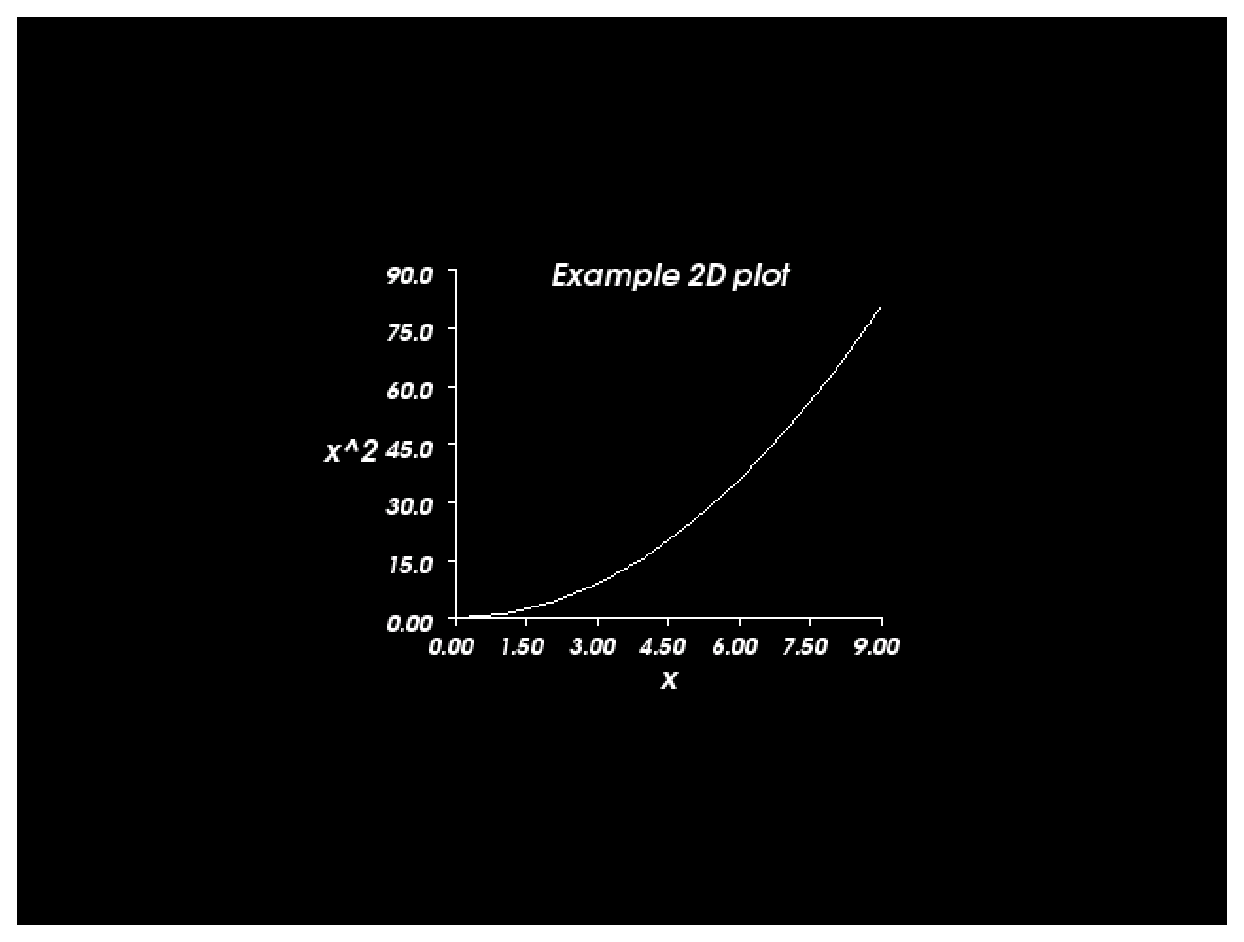
\includegraphics[width=\figwidth]{figures/plotExampleVTK}%
}
\caption{Output from vtk.}
\end{figure}



\part{Reference Manual}
\label{part:languageReference}

% $Id: languageReference.tex,v 1.1 2005/01/12 01:50:54 paultcochrane Exp $

\chapter{Language Reference}
\label{chap:languageRef}



\part{Developer Manual}
\label{part:developerManual}

% $Id: developerManual.tex,v 1.4 2005/02/07 08:09:10 paultcochrane Exp $

\chapter{Developing \pyvisi}
\label{chap:developingPyvisi}

In here should be docs on how people can contribute code, modules, renderers
etc to the pyvisi project.

\chapter{Objects and methods defined at base level}

Developers of \pyvisi renderer modules need to provide the classes, subclasses
and methods described below.  They need to be defined with stub classes or
methods even if that functionality is not supported by the rendering backend.
An error or warning message should be given if the user tries to call these
null methods or classes, however they need to be there for completeness.

The most up to date and complete version of this information is contained on
the \pyvisi web site under the documentation page, and then the API link.

\section{Class structure}

The following figure is the class structure of \pyvisi

\begin{figure}
\centerline{%
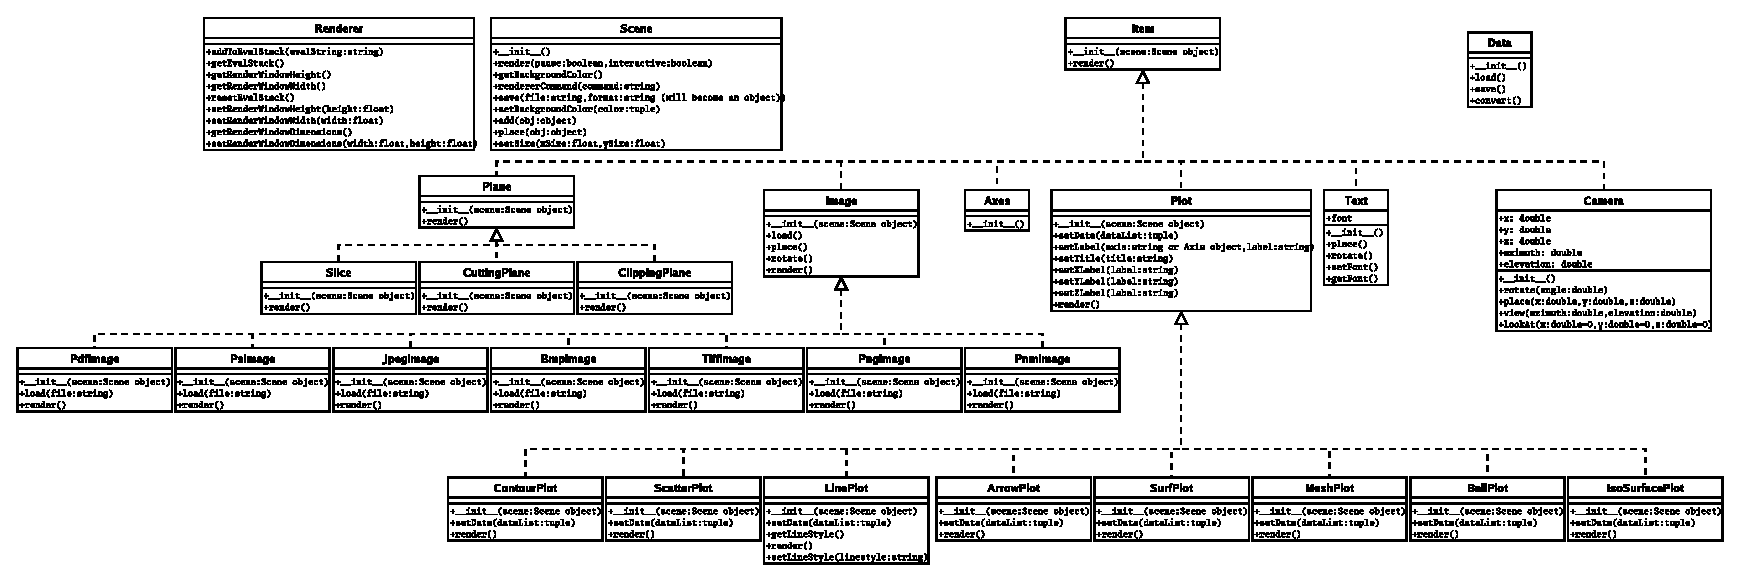
\includegraphics[width=\textheight,angle=90]{figures/pyvisi_class_structure}%
}
\caption{\pyvisi class structure.}
\end{figure}

\section{Fundamental objects}

\subsection{Item}

\subsubsection{render(self)}

Render the object

\subsection{Renderer}

\subsubsection{addToEvalStack(self, evalString)}

Method to add commands to the evaluation stack

\subsubsection{getEvalStack(self)}

Gets the evaluation stack as it currently stands

\subsubsection{getRenderWindowDimensions(self)}

Gets the render window dimensions

\subsubsection{getRenderWindowHeight(self)}

Gets the render window height

\subsubsection{getRenderWindowWidth(self)}

Gets the render window width

\subsubsection{resetEvalStack(self)}

Reset/flush the evaluation stack

\subsubsection{setRenderWindowDimensions(self, width, height)}

Sets the render window dimensions

\subsubsection{setRenderWindowHeight(self, height)}

Sets the render window height

\subsubsection{setRenderWindowWidth(self, width)}

Sets the render window width

\subsection{Scene}

\subsubsection{add(self, obj)}

Add a new item to the scene

\subsubsection{delete(self, obj)}

Delete an item from the scene

\subsubsection{getBackgroundColor(self)}

Gets the current background color setting of the Scene

\subsubsection{getSize(self)}

Gets the current size of the scene

\subsubsection{place(self, obj)}

Place an object within a scene

\subsubsection{render(self, pause, interactive)}

Render (or re-render) the scene

\subsubsection{rendererCommand(self, command)}

Allows the user to run a low-level renderer-specific command directly

\subsubsection{save(self, fname, format)}

Save the scene to a file

\subsubsection{setBackgroundColor(self, *color)}

Sets the background color of the Scene

\subsubsection{setSize(self, xSize, ySize)}

Sets the size of the scene.

\section{Derived objects}

\subsection{Axes}

\subsection{Camera}

\subsection{Image}

\subsubsection{JpegImage}

\subsubsection{PdfImage}

\subsubsection{PngImage}

\subsubsection{PnmImage}

\subsubsection{PsImage}

\subsubsection{TiffImage}

\subsection{Plane}

\subsection{Plot}

\subsubsection{ArrowPlot}

\subsubsection{ContourPlot}

\subsubsection{LinePlot}

\subsection{Text}


%%%%
\chapter{Renderer modules provided by \pyvisi}

\section{vtk}

In the process of being developed.

\section{gnuplot}

In the process of being developed.

\section{povray}

To come.

\section{plplot}

To come.



\part{Appendix}
\label{part:appendix}

\appendix

\include{gpl}

\part{Bibliography and Index}
\backmatter

\bibliography{pyvisi_doc}
%\printindex

\end{document}

